\subsection{Discussion and Analysis}
\label{sec:discuss}

\KQ{
This section compares and contrasts the ODL based model
with other baselines approaches in the end-to-end extraction task.
Based on the results shown in \tabref{tab:compare},
we first observe that \textit{Exact Match} baseline is outperformed by
the other approaches by a significant margin.
The result is not surprising, due to that exact matching approach is highly
sensitive to the recognition accuracy.
Errors occurring on either the target variable or its surrounding constants
will lead to a matching failure,
and noisy text boxes become another factor to affect the extraction accuracy.
}

\KQ{
The other two baselines,
though marginally outperformed by the ODL-based approach,
still have their own important limitations.
\textit{Zonal OCR} is a typical approach that greatly simplifies
the parsing process, at the expense of intensive human labour.
As shown in \figref{fig:zOCR}, users have to annotate the referent zone
(the red box) for \textit{every} single image, which is inefficient.
Besides, the main assumption of this approach is that relative layouts of texts
are accurate and unchanged among all the images of the same format.
The assumption makes sense, but doesn't always hold.
Misrecognition of the zone is disastrous,
as all the extracted information will be incorrect.
For the \textit{Page Layout} approach,
it also requires the consistent page layout result for images of the same format.
\figref{fig:running-page-layout} gives an example of correct page layout,
however, if the textual zone are recognized incorrectly,
necessary information may be omitted from output.
As shown in \figref{fig:errorpl}, the largest textual zone is imperfectly located,
which leads to error information extraction results.
Although having a relative high accuracy,
the extraction wrapper of this method is rather ad-hoc,
which is more challenging for putting into real use.
}

\KQ{
Compared with those baselines,
the ODL based approach doesn't rely on any carefully defined bounding boxes,
its most important advantage is to make full use of the relative layout
information between expressions embedded in the ODL description.
Based on the implicit layout restrictions,
the parser is able to generate the optimized alignment between
expressions and text boxes, while satisfying both value and spatial constraints.
}
% However, the fuzzy match design of our system can
% tolerate these types of errors that the OCR engine made.
% We seek to find an optimization solution which can extract
% correct information as much as possible.


\begin{figure*}[ht]
\centering
\epsfig{file=figure/error_page_layout.eps, width=1.9\columnwidth}
\caption{Example result of an imperfect page layout analysis.}
\label{fig:errorpl}
\end{figure*}
